\PassOptionsToPackage{unicode}{hyperref}
\documentclass[aspectratio=1610, 9pt]{beamer}

% Load packages you need here
\usepackage{polyglossia}
\setmainlanguage{german}

\usepackage{csquotes}
\usepackage{graphicx}
\usepackage{siunitx}
\usepackage{amsmath}
\usepackage{amssymb}
\usepackage{mathtools}

\usepackage{hyperref}
\usepackage{bookmark}

% load the theme after all packages

\usetheme[
  showtotalframes, % show total number of frames in the footline
   % dark, % optional dark theme, uncomment to use
]{tudo}

% Put settings here, like
\unimathsetup{
  math-style=ISO,
  bold-style=ISO,
  nabla=upright,
  partial=upright,
  mathrm=sym,
}
\begin{document}
\title{Observing the Prompt Component of the Atmospheric Muon Flux Using IceCube}
\author{Leander Flottau}
%\institute{Astroteilchenphysik \\  Fakultät: Physik}
\titlegraphic{
\includegraphics[width=0.7\textwidth]{Plots/IceCube_webheader_fullcolor}}
\begin{document}
\maketitle
%\begin{frame}
%  \frametitle{Table of Contents}
%  \tableofcontents
%\end{frame}  
%\section{IceCube Neutrino Observatory}
\begin{frame}
    \frametitle{IceCube Neutrino Observatory}
    \begin{minipage}{0.6\textwidth}
        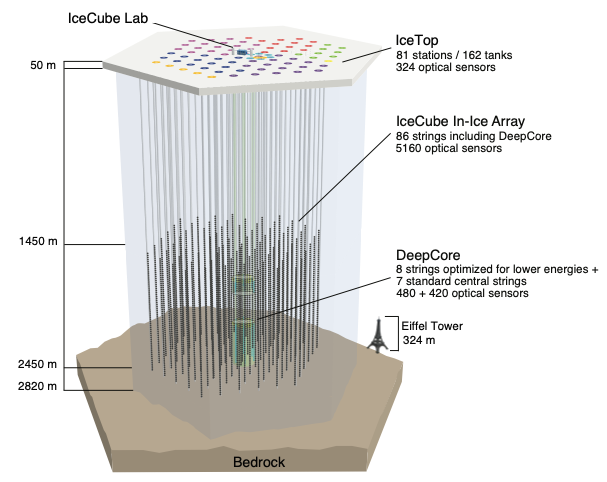
\includegraphics[width=\textwidth]{Plots/IceCube schematic}
    \end{minipage}
    \begin{minipage}{0.39\textwidth}
        \begin{itemize}
            \item Cubic kilometer scale cherenkov detector
            \item $5160$ DOMs on $86$ strings
            %\item ~$270$ measured neutrino Events per day
            \item ~$\approx \SI{3}{\kilo\hertz}$ muon event rate
        \end{itemize}
    \end{minipage}
\end{frame}
\begin{frame}
    \frametitle{Atmospheric Air Showers}
    \begin{minipage}{0.6\textwidth}
        \includegraphics[width=\textwidth]{Plots/Air Shower Illustration}
    \end{minipage}
    \begin{minipage}{0.39\textwidth}
        \begin{itemize}
            \item Cosmic ray interactions produce secondary particles
            \item Major decay product: $\mu$
        \end{itemize}
    \end{minipage}
\end{frame}
\begin{frame}
    \frametitle{The Prompt Component}
    \begin{minipage}{0.6\textwidth}
        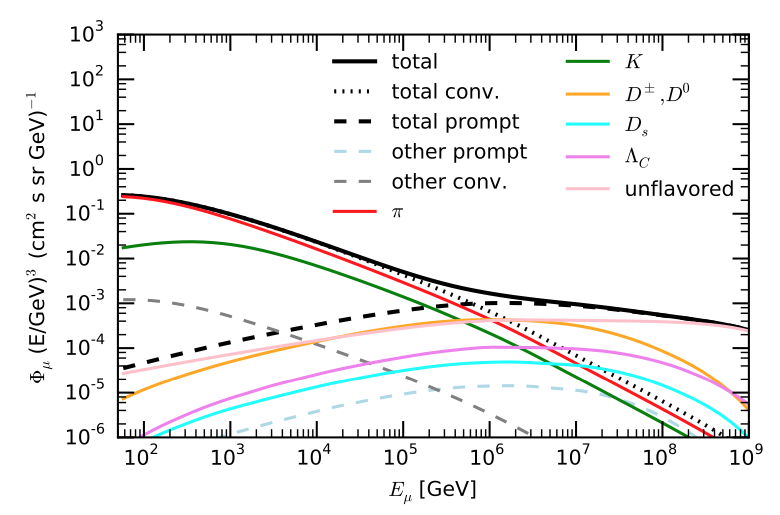
\includegraphics[width=\textwidth]{Plots/Prompt vs conventional flux}
    \end{minipage}
    \begin{minipage}{0.39\textwidth}
        \begin{itemize}
            \item Conventional: produced by $K^{\pm}$/$\pi^{\pm}$
            \item Prompt: produced by short lived particles
            \item Prompt dominant at high energies
        \end{itemize}
    \end{minipage}
\end{frame}
\begin{frame}
    \frametitle{The Muon-Puzzle}
    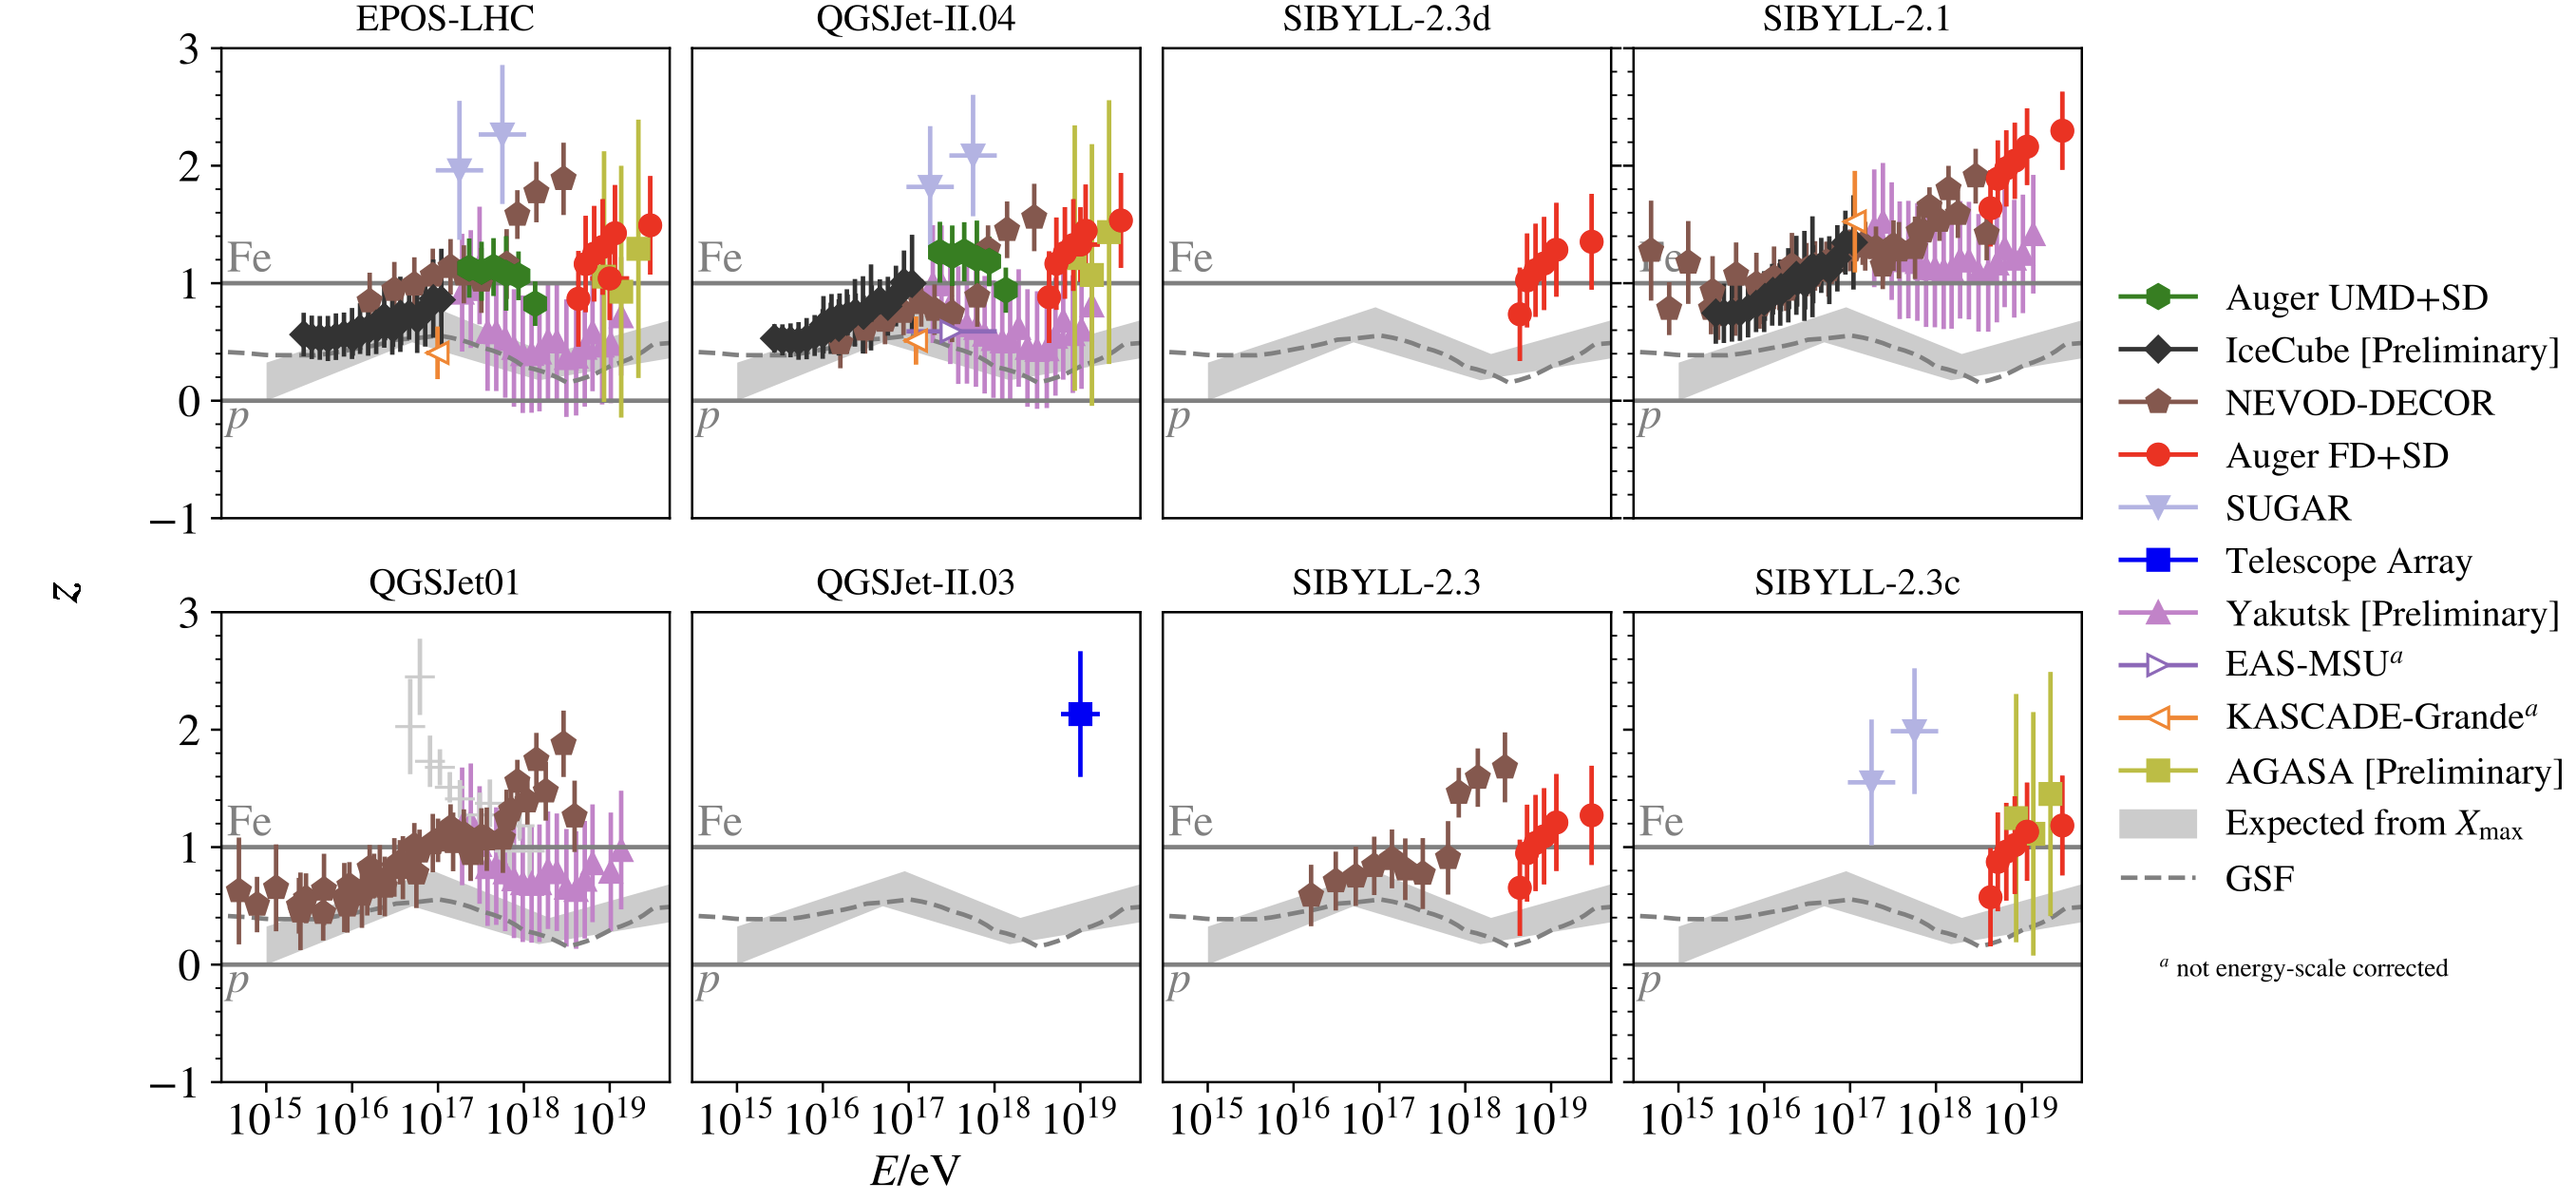
\includegraphics[width=0.9\textwidth]{Plots/muon puzzle}
%    \begin{itemize}
%        \item More muons measured than simulations predicted
%        \item Hadronic interaction models
%    \end{itemize}
\end{frame}
\begin{frame}
    \frametitle{Simulations and tagging}
    \begin{itemize}
        \item Tagging of parent particles in CORSIKA simulations
        \item Prompt definition based on parent of leading muon
        \item Allows for MC-Sample with prompt/conventional distinction 
        \item Simulation up to extremely high energies $>\SI{10}{\peta\electronvolt}$
    \end{itemize}
\end{frame}
\begin{frame}
    \frametitle{Reconstructions}
    \begin{itemize}
        \item Neural network based
        \item Zenith angle, bundle energy and leading muon energy
        \item Small network for precuts
    \end{itemize}
\end{frame}
\begin{frame}
    \frametitle{Forward Folding}
    \begin{minipage}{0.6\textwidth}
        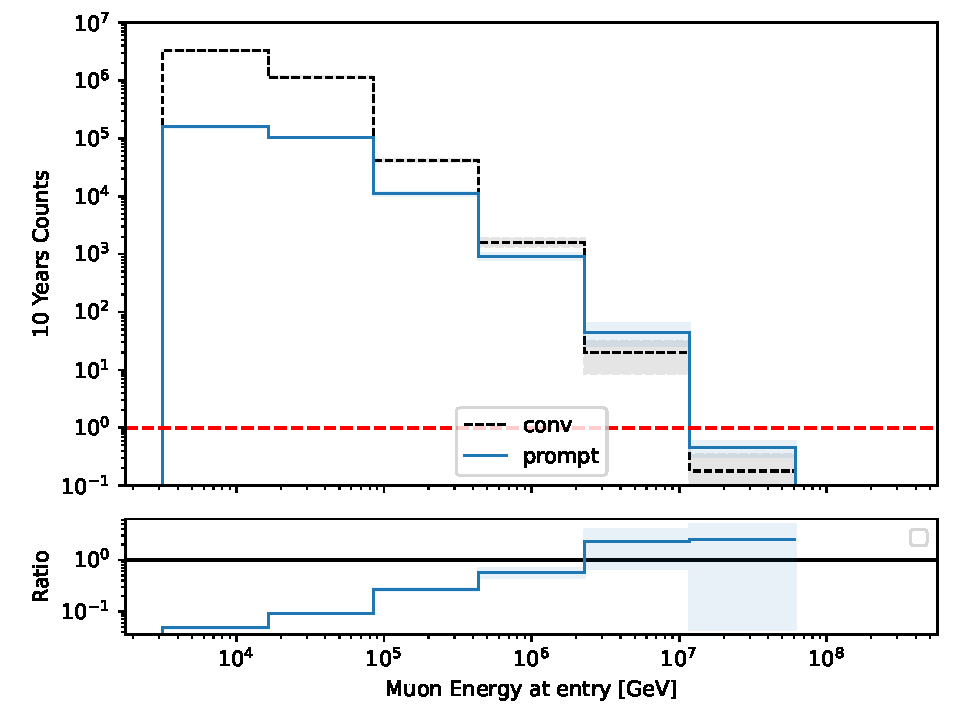
\includegraphics[width=\textwidth]{Plots/spectrum_(3.5,8.5,8)_10Y}
    \end{minipage}
    \begin{minipage}{0.39\textwidth}
        \begin{itemize}
            \item Prompt normalization: fraction of prompt component relative to current MC-simulation $n_p$
            \item Poisson likelihood in each histogram bin
            \item Rescale with normalization factors 
            \item Strong model dependency
        \end{itemize}
    \end{minipage}
\end{frame}
\begin{frame}
    \frametitle{Pseudoexperiments}
    \begin{minipage}{0.6\textwidth}
        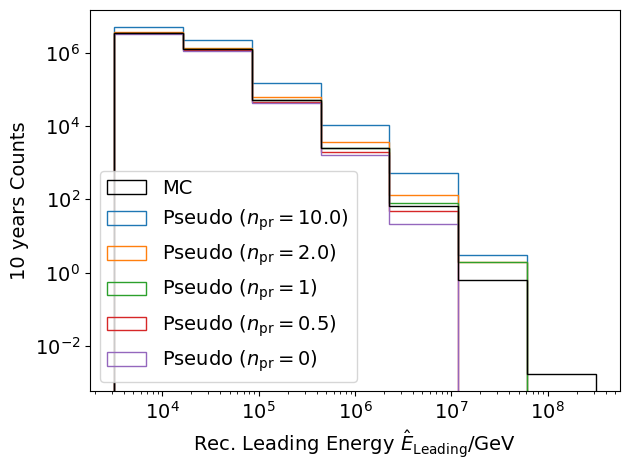
\includegraphics[width=\textwidth]{Plots/injected norms}
    \end{minipage}
    \begin{minipage}{0.39\textwidth}
        \begin{itemize}
            \item Testing methods based on simulations
            \item Events drawn based on primary model and normalizations
            \item Inject normalization
        \end{itemize}
    \end{minipage}
\end{frame}
\begin{frame}
    \frametitle{Background Estimation}
    \begin{minipage}{0.6\textwidth}
        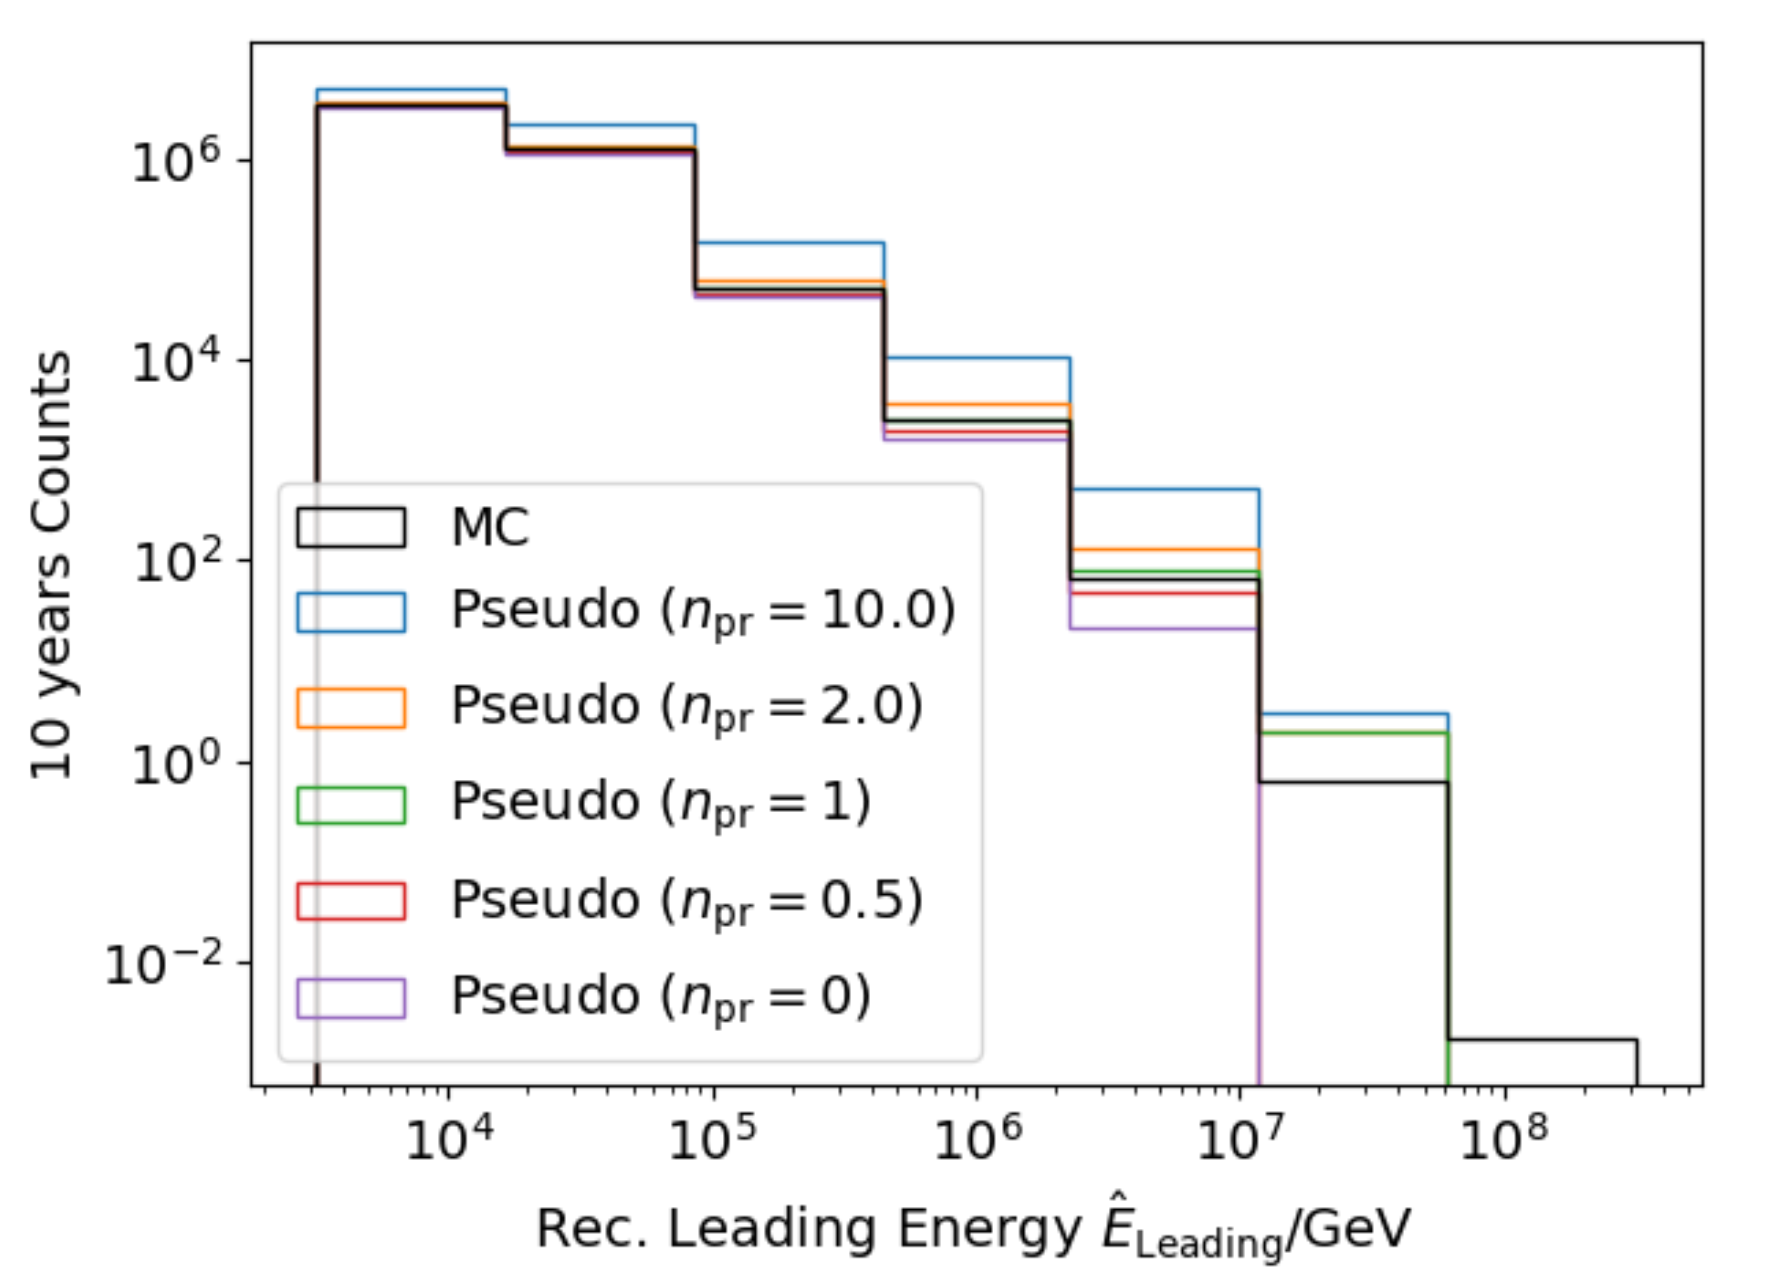
\includegraphics[width=\textwidth]{Plots/background_statistic_chi2_(3.5,8.5,8)_10Y}
    \end{minipage}
    \begin{minipage}{0.39\textwidth}
        \begin{itemize}
            \item Likelihood ratio test
            \item Draw background samples with $n_p=0$
            \item Wilks' theorem: fit $\Chi^2$-distribution
        \end{itemize}
    \end{minipage}
\end{frame}
\begin{frame}
    \frametitle{Discovery Potential}
    \begin{minipage}{0.6\textwidth}
        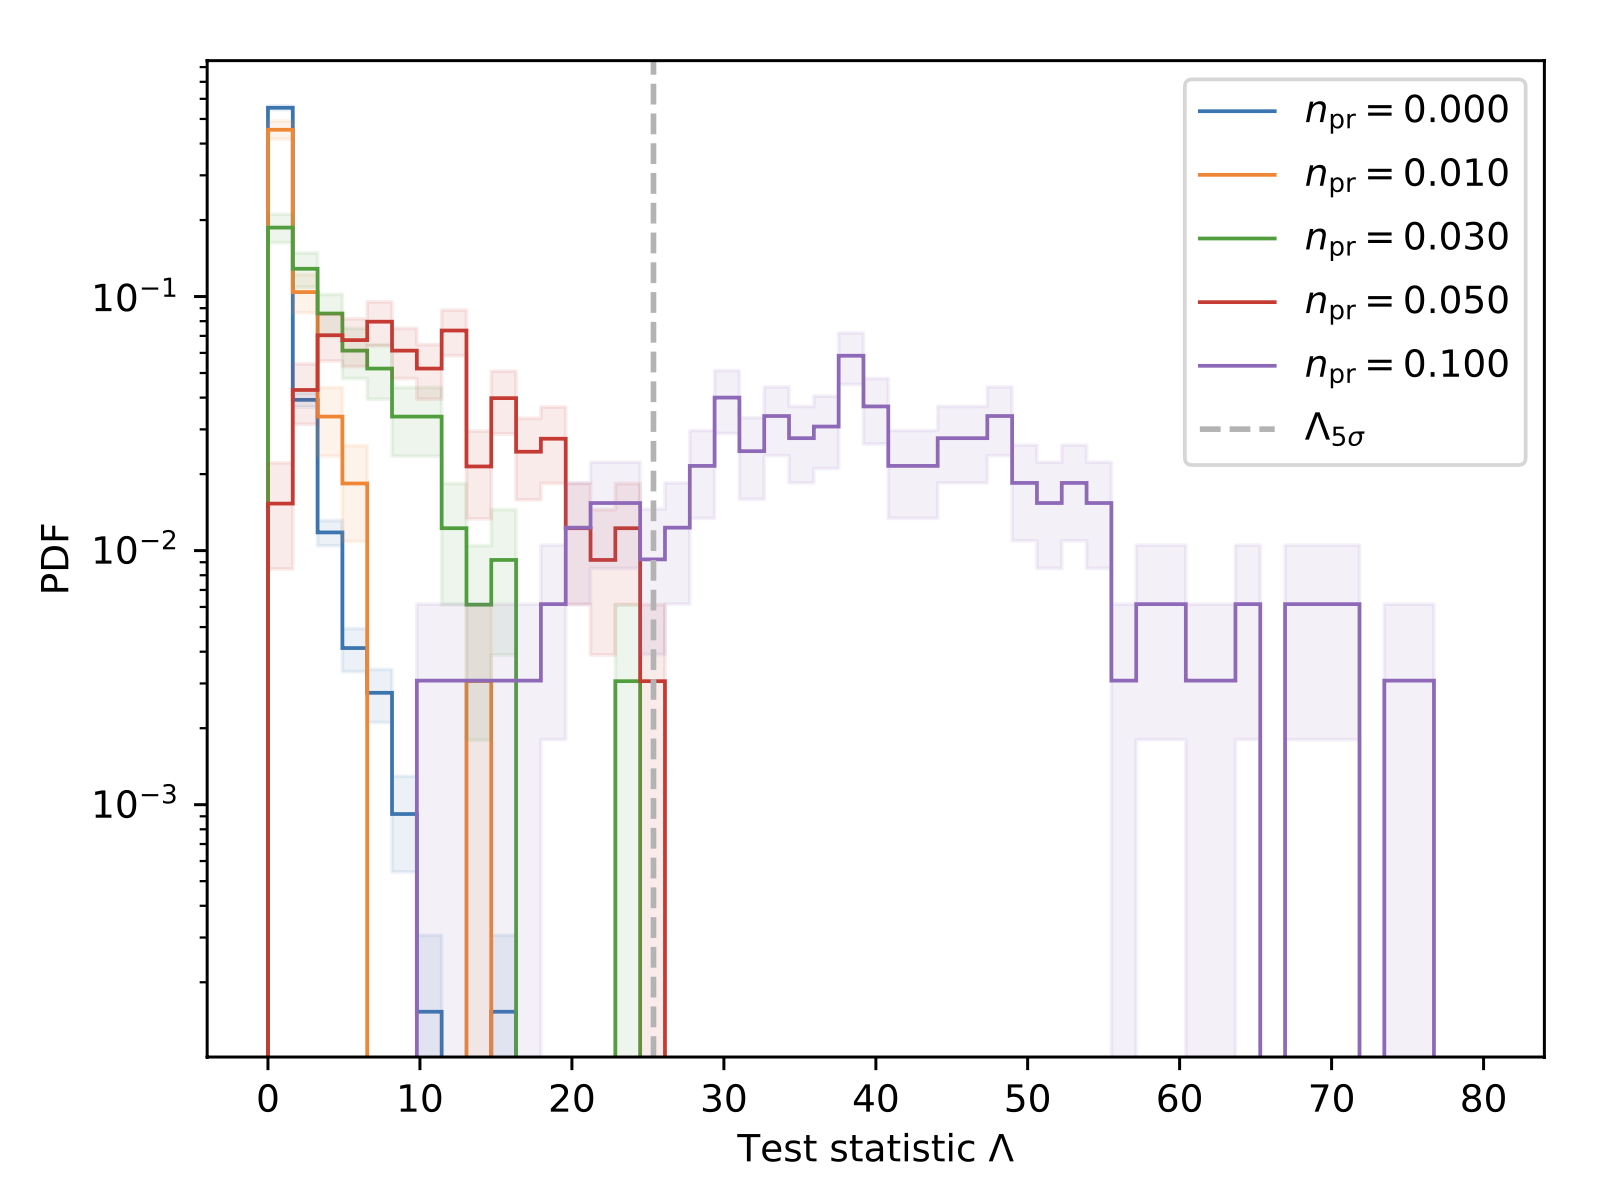
\includegraphics[width=\textwidth]{Plots/TS_Distribution(3.5,8.5,8)_10Y}
    \end{minipage}
    \begin{minipage}{0.39\textwidth}
        \begin{itemize}
            \item How high does the prompt norm have to be to detect it with the current method?
            \item Discovery potential: Norm at which half the generated trials yield $5 \sigma$ significance in the likelihood ratio test
            \item Sensitive to input parameters, binning etc
        \end{itemize}
    \end{minipage}
\end{frame}
\begin{frame}
    \frametitle{Summary}
    \begin{itemize}
        \item Generate prompt tag in simulation
        \item Simulate up to high energies
        \item Forward fit of prompt normalization
        \item Use MC data to estimate significance
    \end{itemize}
\end{frame}
\begin{frame}
    \frametitle{Conclusion}
\end{frame}
\end{document}